\documentclass{article}
\usepackage[utf8]{inputenc}
\usepackage{multicol}
\usepackage{listings}
\usepackage{verbatim}
\usepackage{color}
\usepackage{geometry}
\usepackage{float}
\usepackage{amsmath}

\usepackage{pdflscape}
\usepackage{hyperref}
\setlength{\belowcaptionskip}{-10pt}
\setlength{\abovecaptionskip}{-30pt}
\floatstyle{boxed} 
\restylefloat{figure}
\usepackage{graphicx}
\definecolor{codegreen}{rgb}{0,0.6,0}
\definecolor{codegray}{rgb}{0.5,0.5,0.5}
\definecolor{codepurple}{rgb}{0.58,0,0.82}
\definecolor{backcolour}{rgb}{0.95,0.95,0.92}

\lstdefinestyle{mystyle}{
	backgroundcolor=\color{backcolour},   
	commentstyle=\color{codegreen},
	keywordstyle=\color{blue},
	numberstyle=\tiny\color{codegray},
	stringstyle=\color{codepurple},
	basicstyle=\footnotesize,
	breakatwhitespace=false,         
	breaklines=true,                 
	captionpos=b,                    
	keepspaces=true,                 
	numbers=left,                    
	numbersep=5pt,                  
	showspaces=false,                
	showstringspaces=false,
	showtabs=false,                  
	tabsize=2
}

\lstset{style=mystyle}
\title{Image Processing\\
		Home work 03\\Image Enhancement in Frequency Domain }
\author{Aqeel Labash\\ \textbf{Lecturer:} Gholamreza Anbarjafari}
\date{2 April 2016}

\geometry{
	a4paper,
	total={170mm,257mm},
	left=10mm,
	top=5mm,
}
\begin{document}
	\maketitle
\section*{\centering Filtering Methods in Frequency Domain}
\begin{multicols*}{2}
\section{Low Pass filters}
They are also called blurring filters.\cite{1}
\subsection{Ideal}
In idea low pass filter we put zero for all the frequencies above the cutoff frequencies.So instead of rectangular pulse in 1D it's cylindrical in 2D.\cite{2}\\
So the multiplication matrix is defined as following : 
  \[
  H(u,v)=\left\{
  \begin{array}{ll}
  1 \text{ if } D(u,v)\leq D_0\\
  0 \text{ if } D(u,v)> D_0
  \end{array}
  \right.
  \]
To understand it better here is an example showing the steps:
\begin{figure}[H]
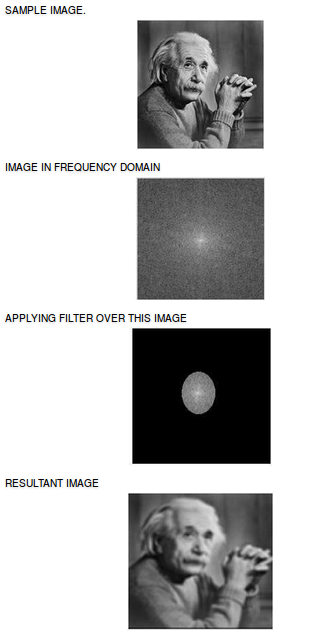
\includegraphics[scale =0.5]{ideallowpass.png}
\end{figure}
In the previous figure we can see the steps and how the frequency domain looks like after applying the filter.We saw also how the image become after we do the Fourier inverse. 
\subsection{Butterworth}
Butter worth :"designed to have as flat a frequency response as possible in the passband"\cite{3}.
In butter worth we generate the multiplication matrix with the following formula :
\[H(u,v)=\frac{1}{1+[\frac{D(u,v)}{D_0}]^{2n}}\]
In this way will have smooth change not 1 or 0 value. So The more far we are from \(D_0\) the more close the value to zero.
\subsection{Gaussian}
The multiplication matrix is definded by the following formula : 
\[ H(u,v) = e^{\frac{-D^2(u,v)}{2D_0^2}} \]	
Gaussian filter in general (low pass or high pass ) solve the Ideal filter ringing problem.That's because if we noticed the formula we can see that's it's gradually change not working as switch on/off.
\section{High Pass filters}
The are also called derivative filters.\cite{1}
\subsection{Ideal}
It's exactly the opposite of Ideal low pass filter where it allow the filters with high frequencies to pass and prevent other frequencies.Next figure shows an example of how the multiplication matrix looks like :
\begin{figure}[H]
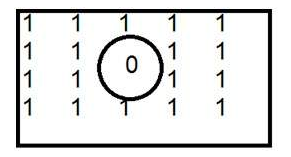
\includegraphics[scale=0.5]{ihpfexample.png}
\caption{Shows example of how H(u,v) matrix would look like}
\end{figure}
The formula for \(H(u,v)\) is defined:
  \[
  H(u,v)=\left\{
  \begin{array}{ll}
  0 \text{ if } D(u,v)\leq D_0\\
  1 \text{ if } D(u,v)> D_0
  \end{array}
  \right.
  \]
\subsection{Butterworth}
The multiplication matrix is given by the following formula:
\[H(u,v)=\frac{1}{1+[\frac{D_0}{D(u,v)}]^{2n}}\]
If we look more to the formula we can see it's the same as Butterworth for low pass frequency after reversing \(D_0, D(u,v)\) places which will allow us to reverse the behavior of the filter to pass the high frequencies.
\subsection{Gaussian}
As I wrote earlier Gaussian filter in general (low pass or high pass ) solve the Ideal filter ringing problem. \(H(u,v)\) is given by the following formula :
\[ H(u,v) =1- e^{\frac{-D^2(u,v)}{2D_0^2}}\]
From the previous formula we can notice that we are taking the complement value and we can write as : 
\[H(u,v) = 1- GLPF\]
Where GLPF = Gaussian low pass filter.
\end{multicols*}
\section{Implementation Part}
\begin{figure}[H]
	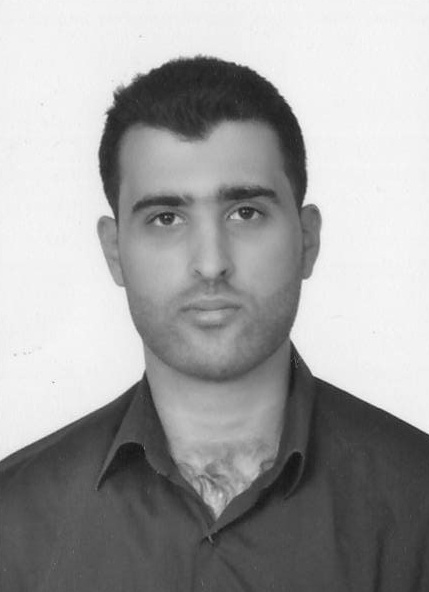
\includegraphics[scale=0.5]{mypicture.jpg}
	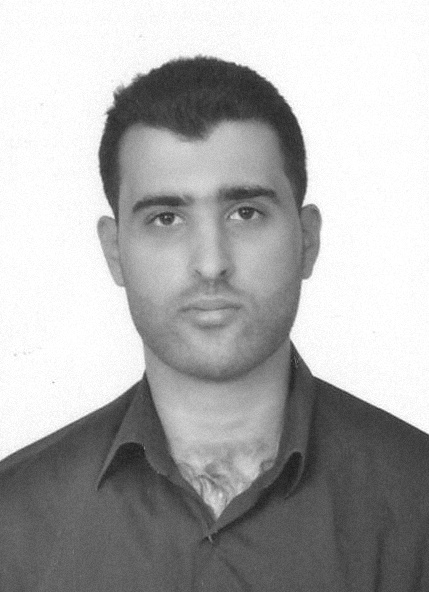
\includegraphics[scale=0.5]{mypic_noised.jpg}
	\caption{Left : orignal , Right: Gaussian noised picture}
\end{figure}
The code used to implement Gaussian noise the image is here : 
\begin{lstlisting}[language=Python]
def NoiseImage(img):
my_nois = np.reshape(np.random.randint(5,20,img.shape[0]*img.shape[1]),(img.shape[0],img.shape[1]))
return Fiximage(img+my_nois)
\end{lstlisting}

\begin{figure}[H]
	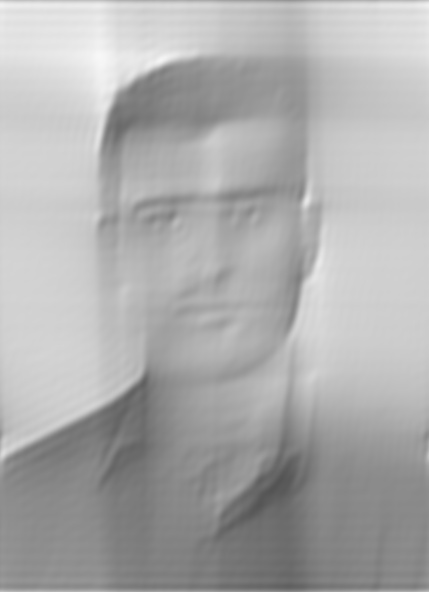
\includegraphics[scale=0.5]{mypic_ILPF.jpg}
	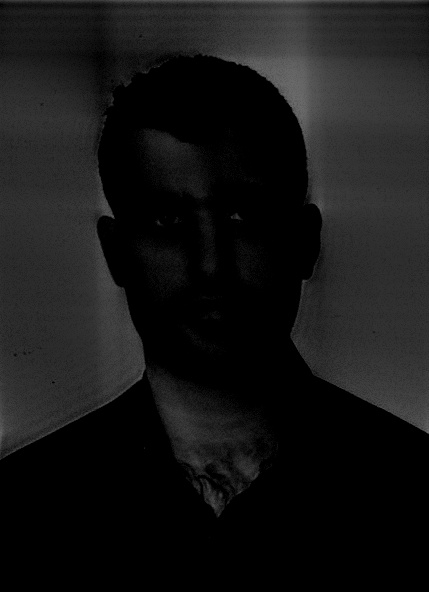
\includegraphics[scale=0.5]{mypic_IHPF.jpg}
	\caption{Left : Ideal low pass filter , Right: ideal high pass filter}
\end{figure}
\begin{lstlisting}[language=Python]
def distance(u,v):
return np.sqrt(pow(float(u),2)+pow(float(v),2))

def ILPF(img,d0):
imginFD = np.fft.fft2(img)
for i in range(imginFD.shape[0]):
for j in range(imginFD.shape[1]):
imginFD[i,j]*=distance(i,j)<=d0

return  np.array(np.fft.ifft2(imginFD),dtype=int)

def IHPF(img,d0):
imginFD = np.fft.fft2(img)
for i in range(imginFD.shape[0]):
for j in range(imginFD.shape[1]):
imginFD[i,j]*=distance(i,j)>=d0

return  np.array(np.fft.ifft2(imginFD),dtype=int)
\end{lstlisting}
\begin{figure}[H]
	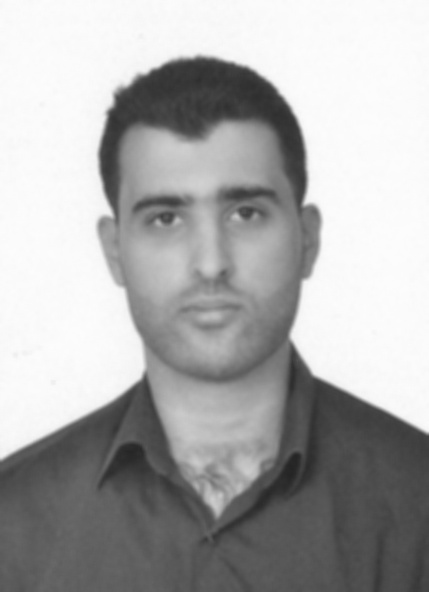
\includegraphics[scale=0.5]{mypic_GLPF.jpg}
	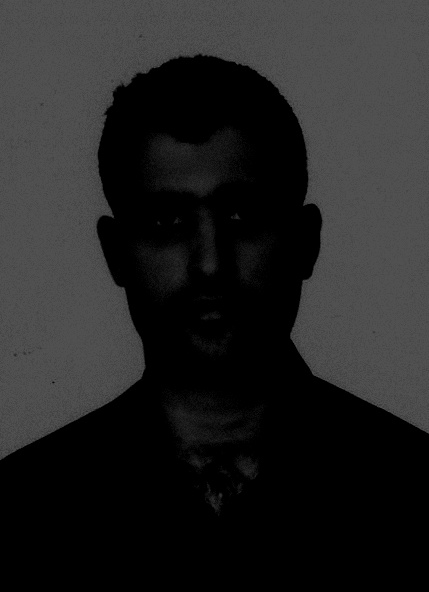
\includegraphics[scale=0.5]{mypic_GHPF.jpg}
	\caption{Left : Gaussian low pass filter , Right: Gaussian high pass filter}
\end{figure}
The code used for the previous images : 
\begin{lstlisting}[language=Python]
def GHPF(img,d0):
imginFD = np.fft.fft2(img)
imginFD= np.array(imginFD,dtype=complex)
for i in range(imginFD.shape[0]):
for j in range(imginFD.shape[1]):
imginFD[i,j]*=1-exp(-pow(distance(i,j),2)/2*d0)

return  np.array(np.fft.ifft2(imginFD),dtype=int)

cv2.imwrite('mypic_GHPF.jpg',GHPF(noisedimage,50))
cv2.imwrite('mypic_GLPF.jpg',cv2.GaussianBlur(noisedimage,(5,5),20))
\end{lstlisting}
\begin{thebibliography}{9}
	\bibitem{1}
	\href{http://www.tutorialspoint.com/dip/high_pass_vs_low_pass_filters.htm}{high pass vs low pass filters}
	\bibitem{2}
	\href{http://paulbourke.net/miscellaneous/imagefilter/}{image filters}
	\bibitem{2}
	\href{https://en.wikipedia.org/wiki/Butterworth_filter}{Butterworth filter}
	
	
\end{thebibliography}
\end{document}